\documentclass{article}

\usepackage{geometry}
\geometry{margin=2cm}
\usepackage{graphicx}
\usepackage{hyperref}

\hypersetup{colorlinks=true, linkcolor=blue, urlcolor=blue}
\urlstyle{same}
\begin{document}
	
	\author{Aayush Arya}
	\date{(Submitted: \today)}
	\title{}
	
	\maketitle
	
	\hrule
	\begin{center}
		PHY382 Lab Report\\
		Practical: 1\quad Registration No.: 11912610 \quad Section: G2903
	\end{center}
	\hrule
	
	\section*{Aim}
	To calculate square root of a complex number using \textsc{SciLab}
	
	\section*{Methods}
	We use the \textit{complex}() function to declare a complex variable and the function \textit{sqrt}() to take its square root.\\
	
	As an example, we use the complex number $z = 3 +3i$. An equivalent form of it would be $z=3 \sqrt{2} \left( \frac{1}{\sqrt{2}} + \frac{1}{\sqrt{2}}i \right)$
	
	which, in polar form, is the same as $z = 3\sqrt{2}e^{i\pi/4}$. One can compute its square root by making use of deMoivre's theorem $$(e^{i\theta})^n = e^{in\theta}$$
	
	which implies
	
	$$ z^{1/2} = (3\sqrt{2})^{1/2}e^{i\pi/8}$$
	
	A numerical computation of $e^{i\pi/8}$ by hand is somewhat tedious. We present the output of the same computation being done using SciLab in the succeeding section.
	
	\section*{Results}
	The code and the output are shown in Figure \ref{fig:sqrt}.

	\begin{figure}[h!]
		\centering
		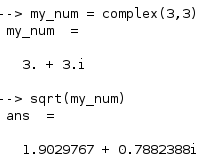
\includegraphics{sqrt_complex}
		\caption{Square root of $z=3+3i$ computed using two lines of code in \textsc{SciLab}.}
		\label{fig:sqrt}
	\end{figure}
	
	SciLab thus provides a much less mechanistic way to calculate square roots of complex numbers.
	
\end{document}